%************************************************
\chapter{Accelerated Chemical Reaction Optimization using Multi-Task Learning}\label{ch:mtbo} 
%************************************************
This chapter is based on the following paper:

\begin{quote}
    Taylor C*., \textbf{Felton K.}*, Wigh D., Jeraal M., Grainger R., Chessari G., Johnson C., Lapkin A. \textit{ACS Central Science}. "Accelerated Chemical Reaction Optimization using Multi-Task Learning." 2023.

    * Joint first authors.
\end{quote}


\textbf{My contribution}: I developed  the idea of applying multitask Bayesian optimization (MTBO) to reaction optimization, implemented the MTBO strategy in Summit and executed the benchmarking studies. All experimental work was completed by Connor Taylor and is presented here to show MTBO in an experimental setting.

\section{Introduction}

In recent years, there has been an increased interest in the use of automated, self-optimizing continuous flow platforms for the optimization of chemical processes.\cite{Reizman2016a, Fabry2016, Fitzpatrick2016, CortesBorda2016} These platforms use automated reactors and machine-learning algorithms to learn from previous experiments, and thereby choose future experiments that ultimately maximize yield and/or other process objectives. The use of self-optimizing platforms has arisen from the desire for faster reaction optimization, improved process sustainability and cheaper overall process development. The use of these platforms aims to enhance the capabilities of the researcher by removing the need for repetitive and labor-intensive experimentation, allowing them to focus on more challenging tasks. By leveraging algorithms, the platforms utilize only minimal reaction material but gain the most process information possible, making their deployment in fine chemical and pharmaceutical industries very attractive.\cite{Clayton2019, Clayton2020}

Recent work has shown that Bayesian optimization is a particularly powerful tool for self-optimization applications.\cite{Amar2019, Schweidtmann2018, Shields2021} However, in all previous studies, each optimization begins with no \textit{a priori} information about the chemical landscape for the reaction of interest. This protocol therefore requires initial experimental iterations whereby the algorithm is learning about the experimental design space, without any prior information on where the optimal reaction conditions may be. This initial exploration can be expensive in terms of both cost and time, particularly when there may already be data on the broad chemical transformation of interest from previous optimization campaigns. This also opens the methodology to some uncertainty over which initial design strategy to use, such as forms of factorial design or Latin Hypercube sampling (LHS), which will affect the overall experimental budget. \textit{General} well-performing reaction conditions can also be identified for particular reaction classes, as highlighted in recent work by Angello \textit{et al.},\cite{Angello2022} but do not give optimal conditions for specific transformations and cannot account for important parameters such as specific reactor differences, solubility, reaction selectivity, differences in substrate functionality or further adjacent objectives (E-factor, purification, downstream processing etc.). The use of optimization strategies for specific substrates in specific instances is therefore still important for determining optimal yields (or other process outputs).

This work shows the first real-world examples of leveraging previous reaction optimization data for unseen chemical transformations using multi-task Bayesian optimization (MTBO). The framework of MTBO, first introduced by Swerksy \textit{et al.},\cite{Swersky2013} replaces the standard probabilistic model in Bayesian optimization with a multi-task model. As these multi-task models can be trained on data from related tasks, we can therefore utilize data from previously conducted similar reactions - both from the laboratory and from the literature. In this work, we first explore and benchmark the use of MTBO in simulated studies, then exploit the methodology to optimize several pharmaceutically relevant C-H activation reactions using an autonomous flow reactor platform. These experimental case studies were chosen to highlight the effectiveness of MTBO in a medicinal chemistry context through efficient material usage. There are many reports of similar automated workflows in the recent literature where a self-optimization protocol is utilized.\cite{Sans2015, Mateos2019} Our reactor platform is equipped with a liquid handling robot and can optimize both continuous variables (residence time, temperature etc.) \textit{and} categorical variables (solvent, ligand etc.). This ability is seldom reported in the literature (with some notable examples from several research groups),\cite{Reizman2016a, Kershaw2023} likely due to engineering and equipment challenges, but is very important in determining all relevant parameters that influence reaction outcomes. The MTBO algorithm utilized is integrated into the Summit, which was introduced in Chapter \ref{ch:summit}, and represents a powerful data-driven optimization technique that can utilize known reaction data and ultimately lead to savings in material, time and overall cost.



\section{Results and Discussion}

\subsection{Bayesian Optimization to Multi-Task Bayesian Optimization}

As shown in Figure \ref{fig:multitask_overview}, Bayesian optimization (BO) relies on three key components: a probabilistic model, an acquisition function and an optimization algorithm. The probabilistic model is trained using experimental data and acts as a surrogate of the real chemical reaction. Given this probabilistic model, the acquisition function estimates the values of different potential experimental reaction conditions. The optimization algorithm is then used to find the set of experimental conditions that maximizes the acquisition function, and these experimental conditions are hence suggested as the next real experiment to run. The combination of the probabilistic model and the acquisition function enables exploitation of known high-performance areas and exploration of new chemical space. By iteratively executing the suggested experimental conditions, retraining the model and optimizing the acquisition function, the BO protocol progressively identifies the best reaction conditions for the output of interest.

\begin{figure}
    \centering
    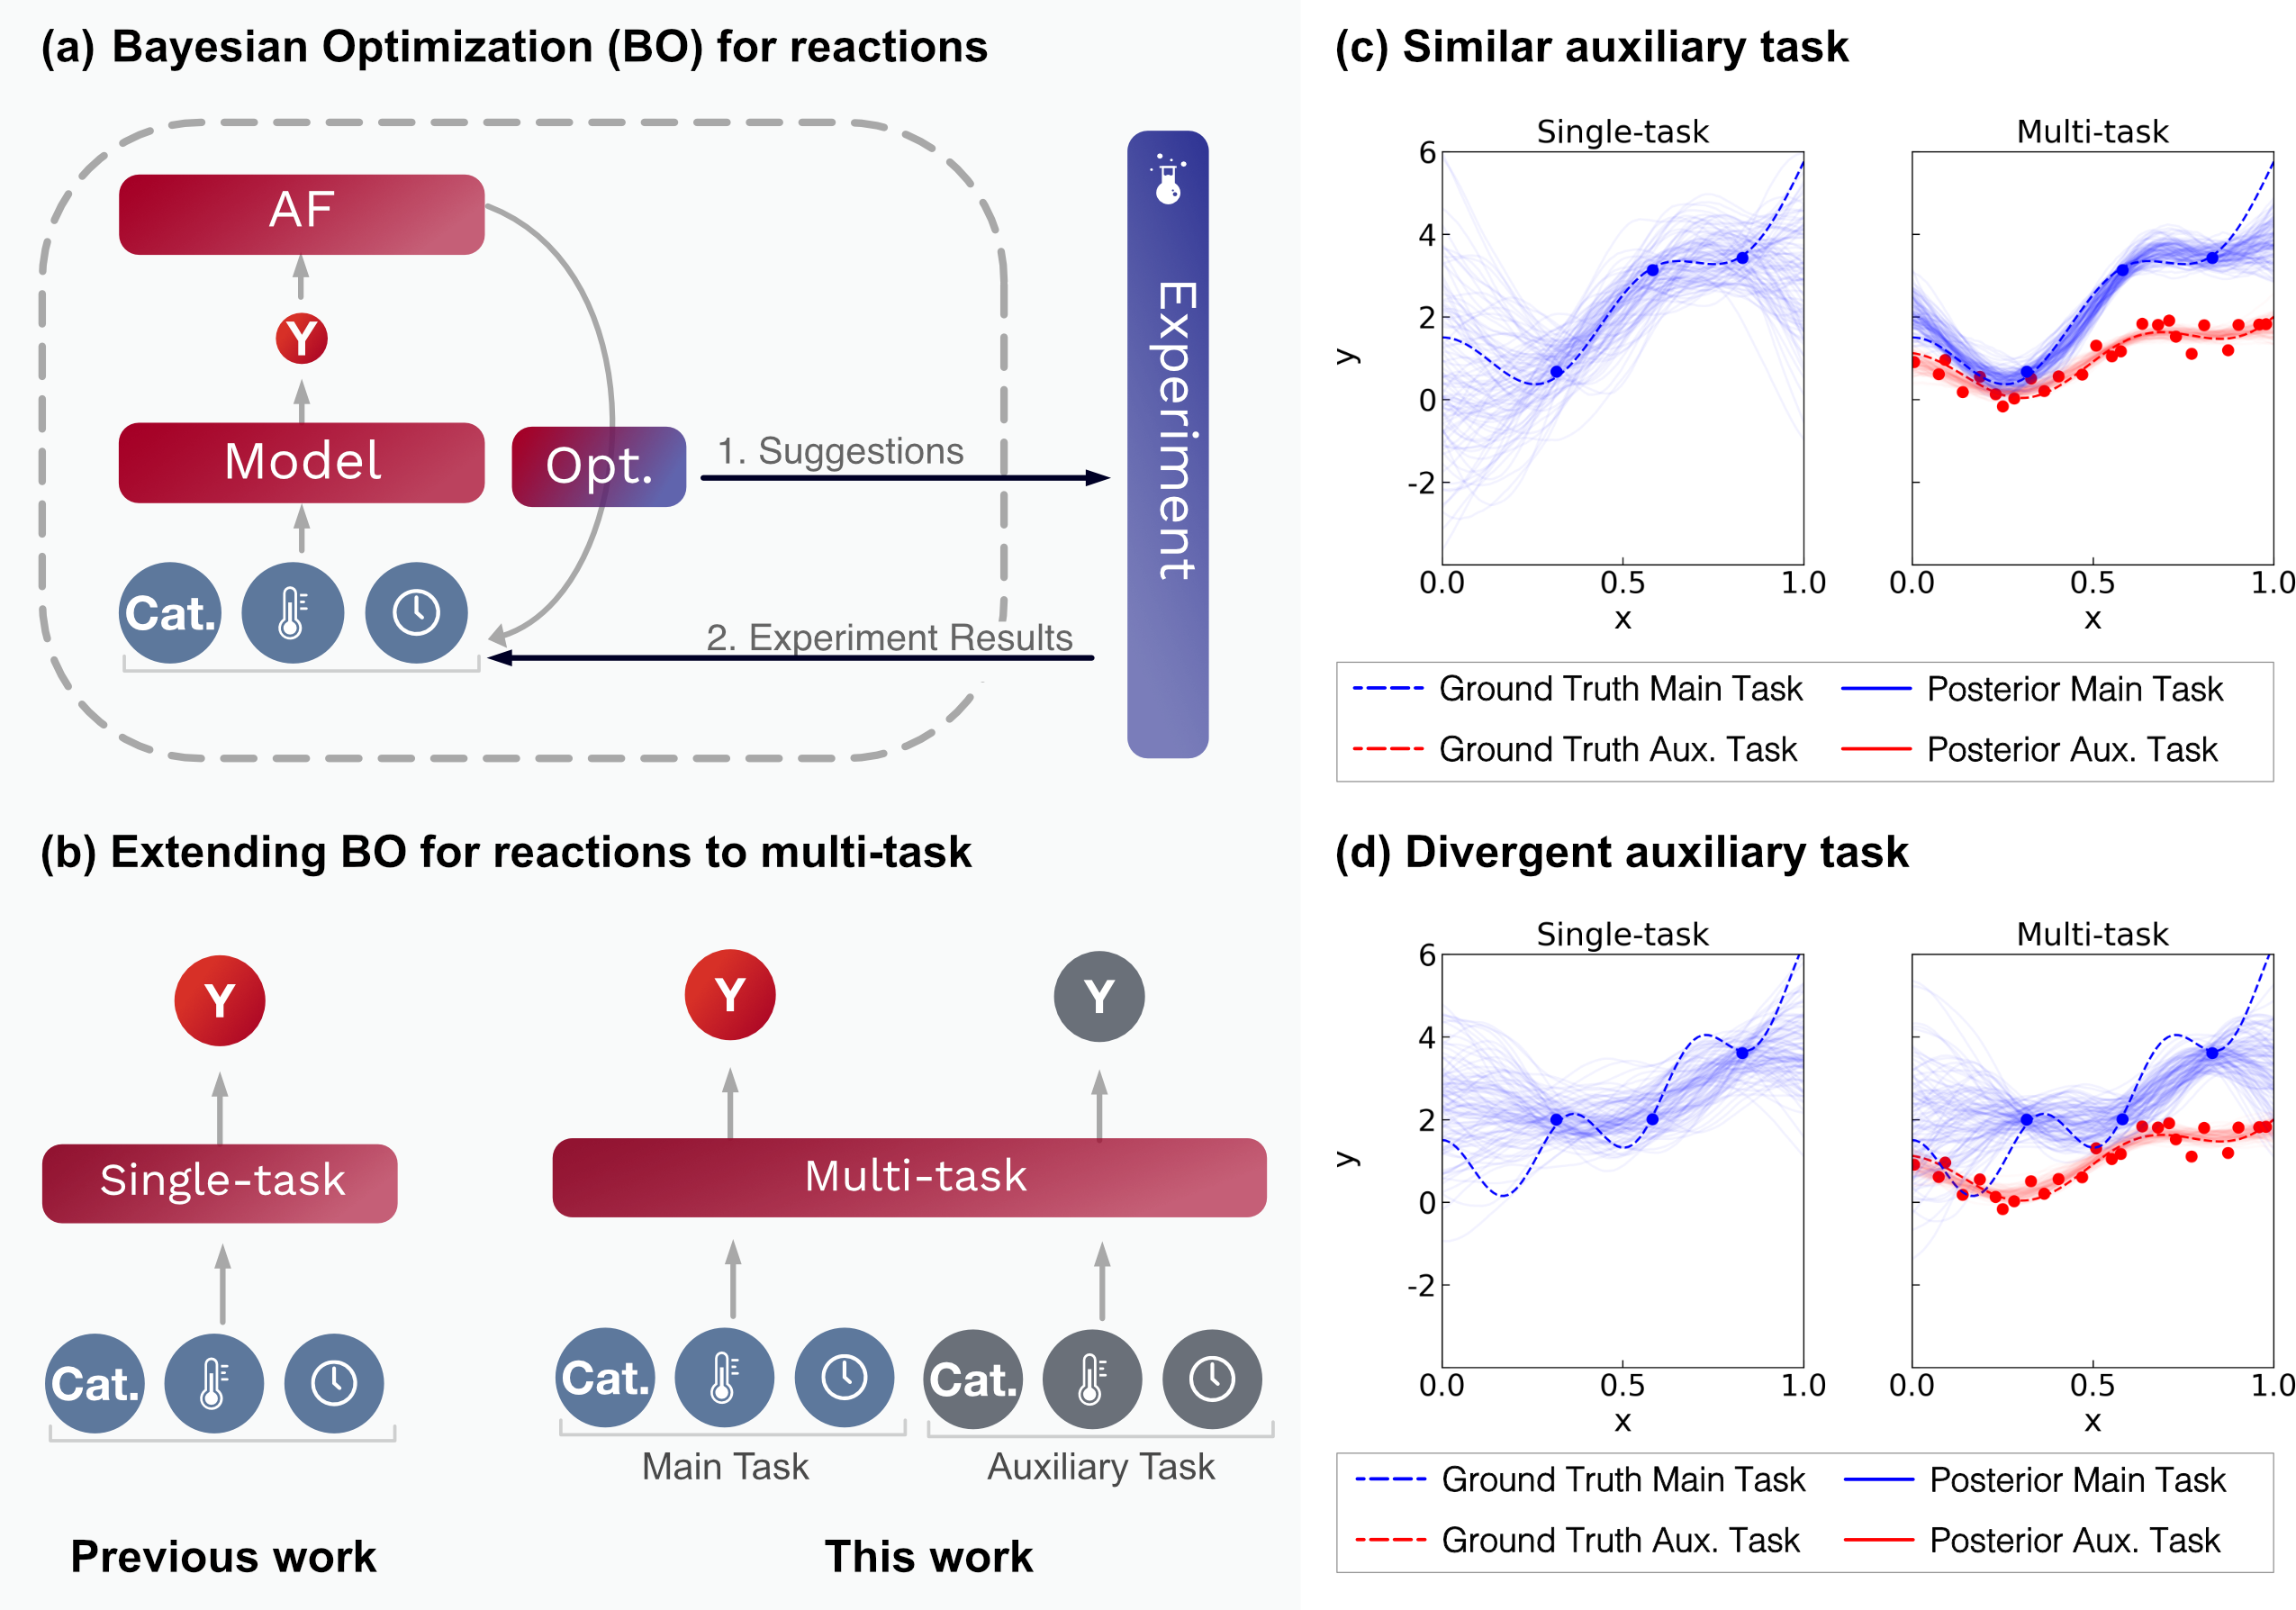
\includegraphics[width=1.2\textwidth]{gfx/Chapter03/paper_figure_1.png}
    \caption{A schematic description of multi-task Bayesian optimization to the context of reaction optimization. (a) Bayesian optimization consists of a probabilistic model (typically a Gaussian process) that predicts experiment outputs (e.g. yield) given experiment conditions; an acquisition function (AF) that predicts the value of potential new experiments; and an optimization algorithm (opt). (b) Multi-task Bayesian optimization replaces the Gaussian process with a multi-task Gaussian process trained simultaneously on an auxiliary task. In our case, this auxiliary task is a similar reaction to the one being optimized, utilizing previous experimental results. (c) When the auxiliary task for a multi-task Gaussian process is similar to the main optimization task, predictions on the main task are improved significantly. (d) When the auxiliary task for a multi-task Gaussian process is divergent to the main optimization task, predictions on the main task are similar to what is observed for the baseline single-task Gaussian process.}
    \label{fig:multitask_overview}
\end{figure}

As shown in Figure \ref{fig:multitask_overview}b, MTBO changes the probabilistic model in BO. Typically, a Gaussian process (GP) is used as the probabilistic model in BO due to the general applicability and efficiency of GPs in the small data regime.\cite{Snoek2012} MTBO replaces a GP with a multi-task GP that can learn the correlations between different tasks to enable better predictions. In our case, the tasks are chemical transformations from the same reaction class with varying substrates. A formal definition of GPs and multi-task GPs is in the Methods section.

As a simple illustration of the benefits of multi-task GPs, we created example functions with one input and one output, then trained both a GP and multi-task GP on only three data points. In the multi-task GP case, we also generated 25 data points from an auxiliary task. As shown in Figure \ref{fig:multitask_overview}c, when the main and the auxiliary tasks are similar, the predictions from the multi-task GP (shown as samples from the posterior of the GP) more accurately represent the underlying function than the predictions from the single-task GP. The multi-task GP leverages covariance between the data in the two tasks to improve predictions on the main task, even with limited data for the main task - this is shown formally in the Methods section. As shown in Figure 1d, when the main and the auxiliary tasks are divergent, predictions from the single-task and multi-task GP are highly variable. However, this variability in the multi-task GP is still useful because the BO algorithm will explore to better capture the underlying distribution of the main task.

\subsection{In Silico Case Studies: Suzuki-Miyaura Couplings}

We first executed \textit{in silico} MTBO studies using model chemical reactions as benchmarks. These models were generated using neural networks trained on literature experimental data that predict reaction yield; more detail on these models can be found in the Methods section. The model `Suzuki B1' was trained using Suzuki cross-coupling data from Baumgartner \textit{et al.},\cite{Baumgartner2018} while the models `Suzuki R1-4' were trained using data from Reizman \textit{et al.}\cite{Reizman2016a}.  These specific transformations and the variables that affect these models are shown in Figure \ref{fig:benchmarks_suzuki}.

\begin{figure}
    \centering
    
\includegraphics[width=0.9\textwidth]{gfx/Chapter03/suzuki_benchmarks_thesis.png}
    \caption{Reaction schemes for the Suzuki cross coupling benchmarks used in this chapter. The data for training the benchmarks are taken from Baumgartner et al. \cite{Baumgartner2018} and \cite{Reizman2016b}. Optimizing these reactions requires tuning continuous variables catalyst loading, reaction time and temperature as Ill as selecting from a library of Buchwald G3 catalysts \cite{Bruno2013}.}
    \label{fig:benchmarks_suzuki}
\end{figure}

Four specific case studies are highlighted in Figure \ref{fig:baumgartner_multitask}, each where the main task is Suzuki B1 and the auxiliary training task is one dataset from each of Suzuki R1-4. In each case study, a conventional single-task Bayesian optimization (STBO) benchmark for the Suzuki B1 reaction serves as a comparison.  An additional baseline, STBO HS, is included which represents starting STBO with the best data from the auxiliary task(s) used for MTBO. For each MTBO study, 96 datapoints from the auxiliary task were utilized. The average best yield for each algorithm is shown with a 95 \% confidence interval over 20 repeated runs. 

\begin{figure}
    \centering
    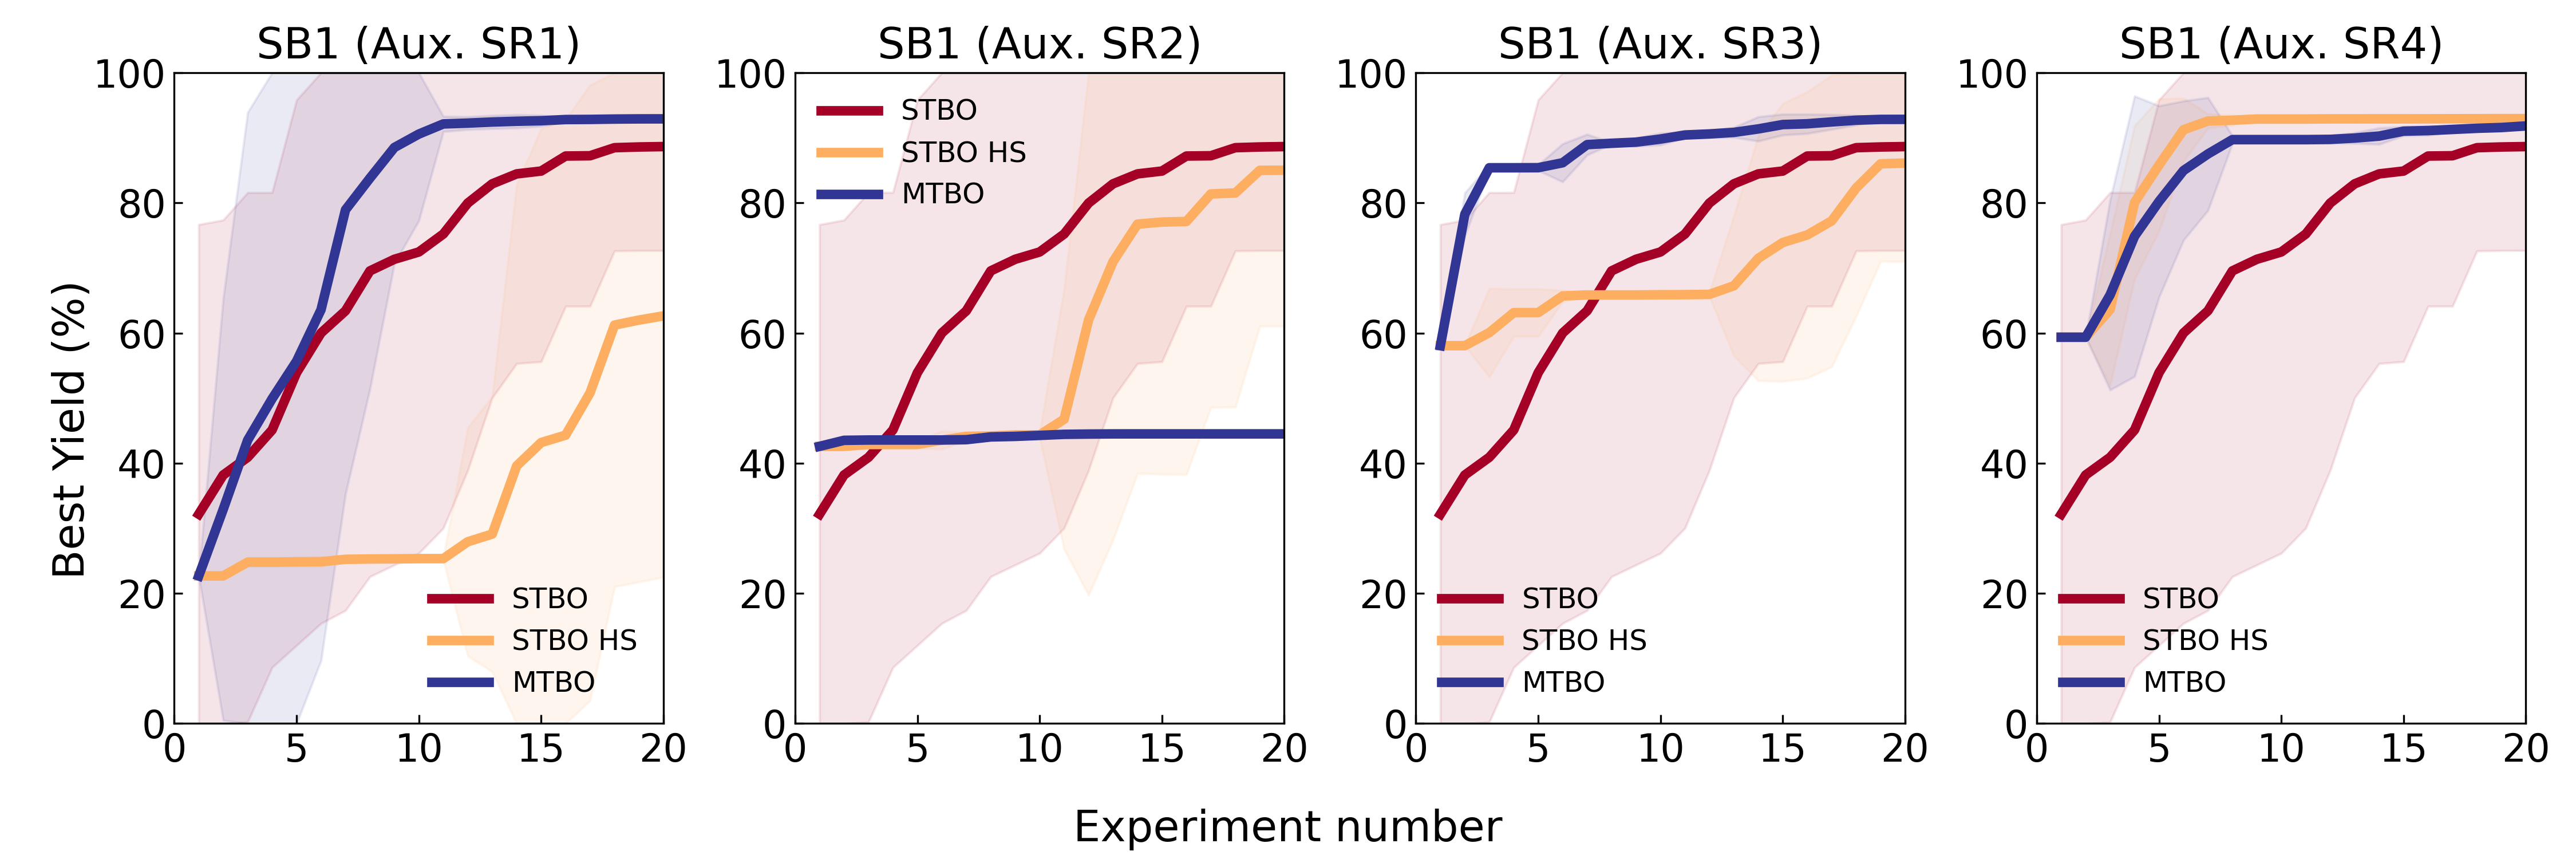
\includegraphics[width=1.2\textwidth]{gfx/Chapter03/baumgartner_suzuki_reizman_suzuki_one_cotraining_optimization.png}
    \caption{A comparison of the performance of single-task Bayesian optimization (STBO) and multi-task Bayesian optimization (MTBO) of Suzuki B1 with Suzuki R1-R4 as auxiliary tasks. The average best yield with a 95 \% confidence interval over 20 repeats is shown. The label above each plot refers to the auxiliary (Aux.) task based on the names in Scheme 1, where Suzuki is abbreviated to S.}
    \label{fig:baumgartner_multitask}
\end{figure}

When leveraging Suzuki R1 as an auxiliary training task, MTBO initially suggests optimal conditions from the training task with P1-L4 (XantPhos). However, these give very low yields (25 \%) which leads to further exploration of the chemical space, resulting in optimal conditions with P1-L1 (XPhos) and a higher yield than STBO. The additional strength shown by MTBO in this case study is the greater speed in obtaining optimal results.

In the second case study, when the auxiliary task is Suzuki R2, MTBO appears to perform poorly - this is likely due to the low reactivity observed in Suzuki R2 and a noisy simulation benchmark (see Figure S8). In this case, the best conditions from the training task also do not perform well on the main task, but the yield is moderate enough that it makes further exploration of the chemical space initially difficult in obtaining a better response. This suggests that MTBO may bias the training data in these circumstances when higher yields are possible but not expected, when given very low-yielding auxiliary tasks. 

In the case studies where the auxiliary tasks were Suzuki R3-4, the reactivity of the substrates was much more similar in both the main and the training tasks, leading to similar optimal conditions being found. This means that MTBO achieved better, and much faster, results than STBO in these cases. 

STBO HS has variable performance relying heavily on the initial conditions it is started with. Overall, we observe that MTBO is less sensitive to changes in optima than MTBO, but MTBO is more sensitive to getting stuck in local optima that might be far away from the condition used initially. 

Performance of MTBO can be greatly improved using \textit{multiple} auxiliary tasks. As shown in Figure \ref{fig:baumgartner_suzuki_reizman_suzuki_all_cotraining_optimization}a, when Suzuki B1 is optimized with Suzuki R1-R4 as auxiliary tasks, the optimal conditions are always found by MTBO in fewer than five experiments. Both P1-L1 and P2-L1 are considered optimal for this reaction, and MTBO selects these two catalysts in over 80 \% of experiments during twenty repeats, when compared to \textless{} 50 \% frequency for STBO - this is highlighted in Figure \ref{fig:baumgartner_suzuki_reizman_suzuki_all_cotraining_optimization}b. As MTBO utilizes optimal regions of chemical space that have been identified in previous tasks with similar reactivity, this allows the algorithm to identify new (and better performing) optimal reaction conditions faster.

\begin{figure}
    \centering
    \begin{subfigure}
        % [c]{0.49\textwidth}
        \centering
        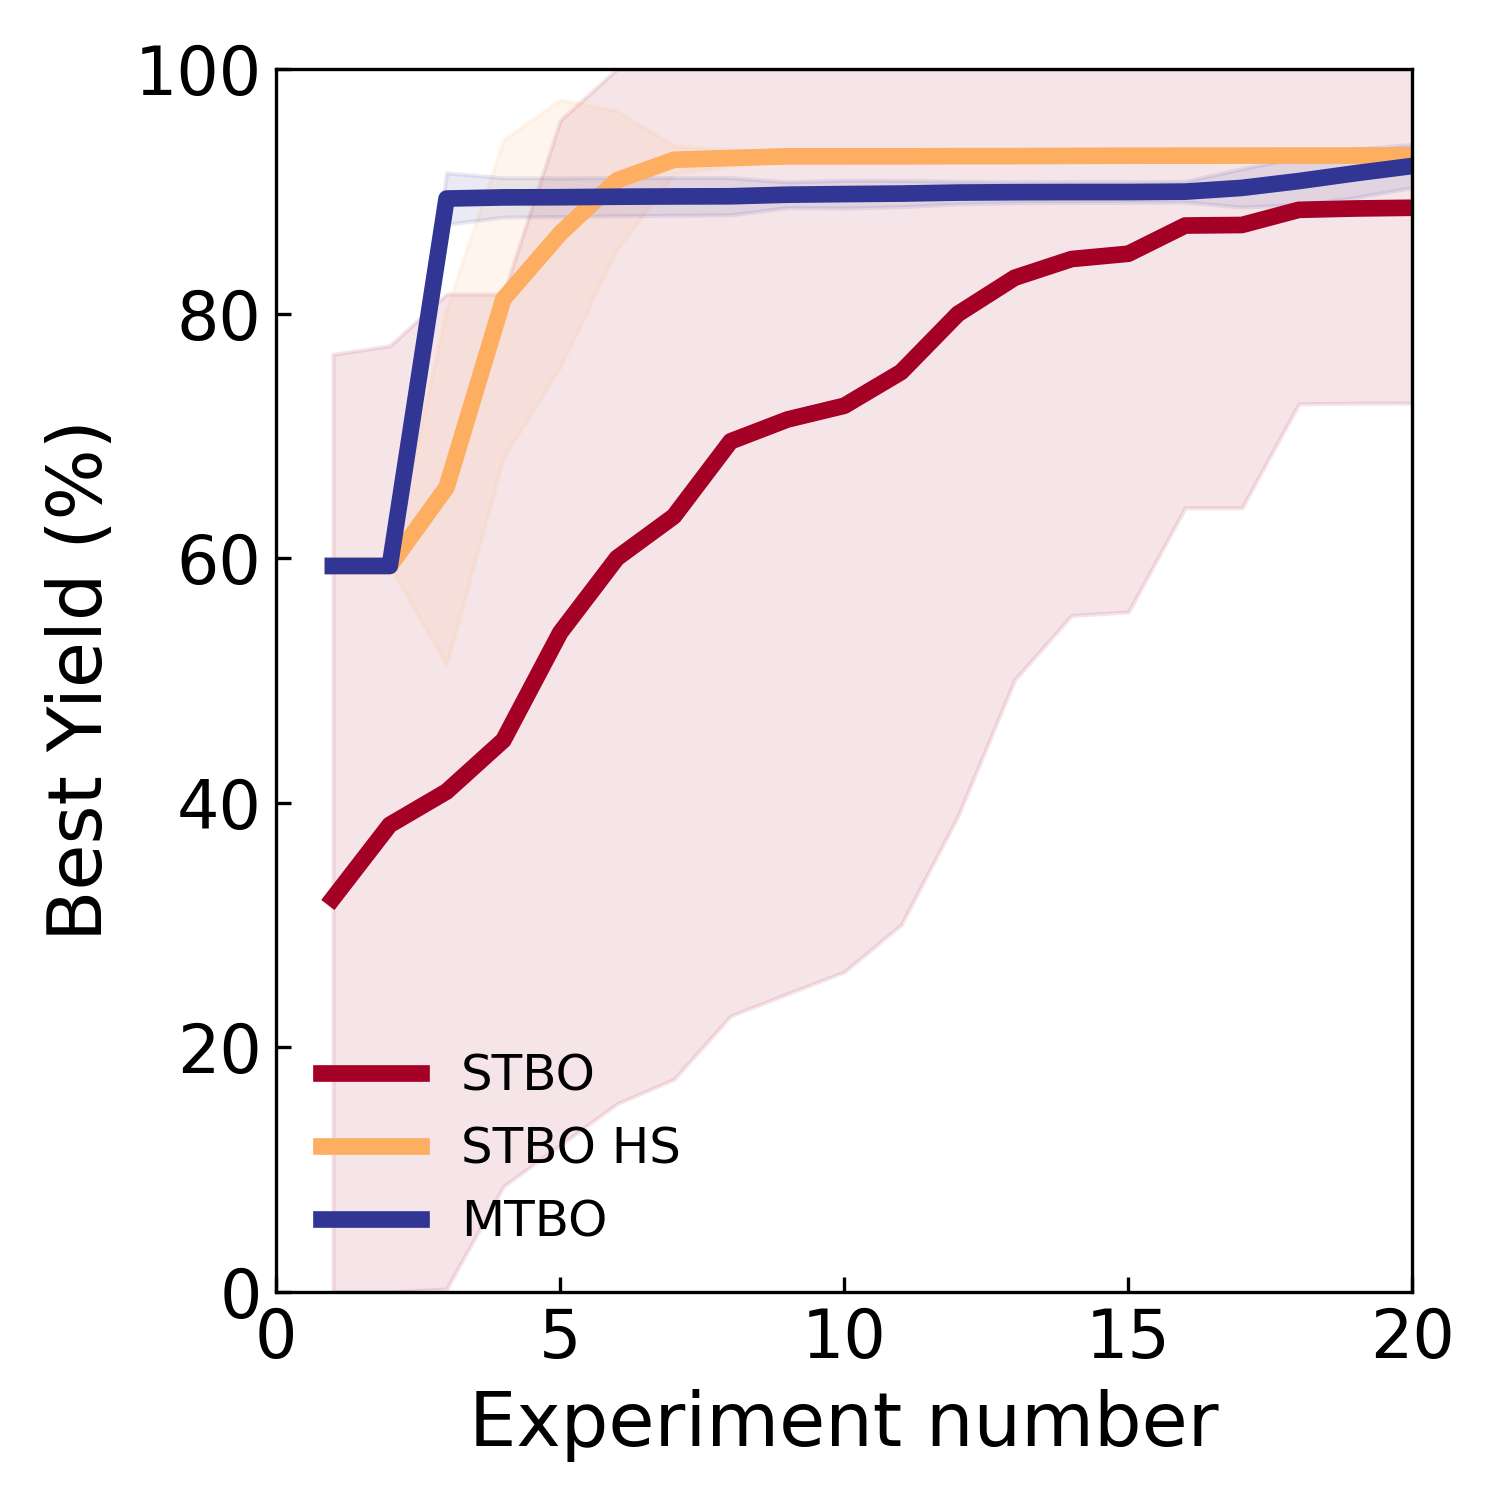
\includegraphics[width=0.8\linewidth]{gfx/Chapter03/baumgartner_suzuki_reizman_suzuki_all_cotraining_optimization.png}
    \end{subfigure} 
    \begin{subfigure}
        % [c]{0.49\textwidth}
        \centering
        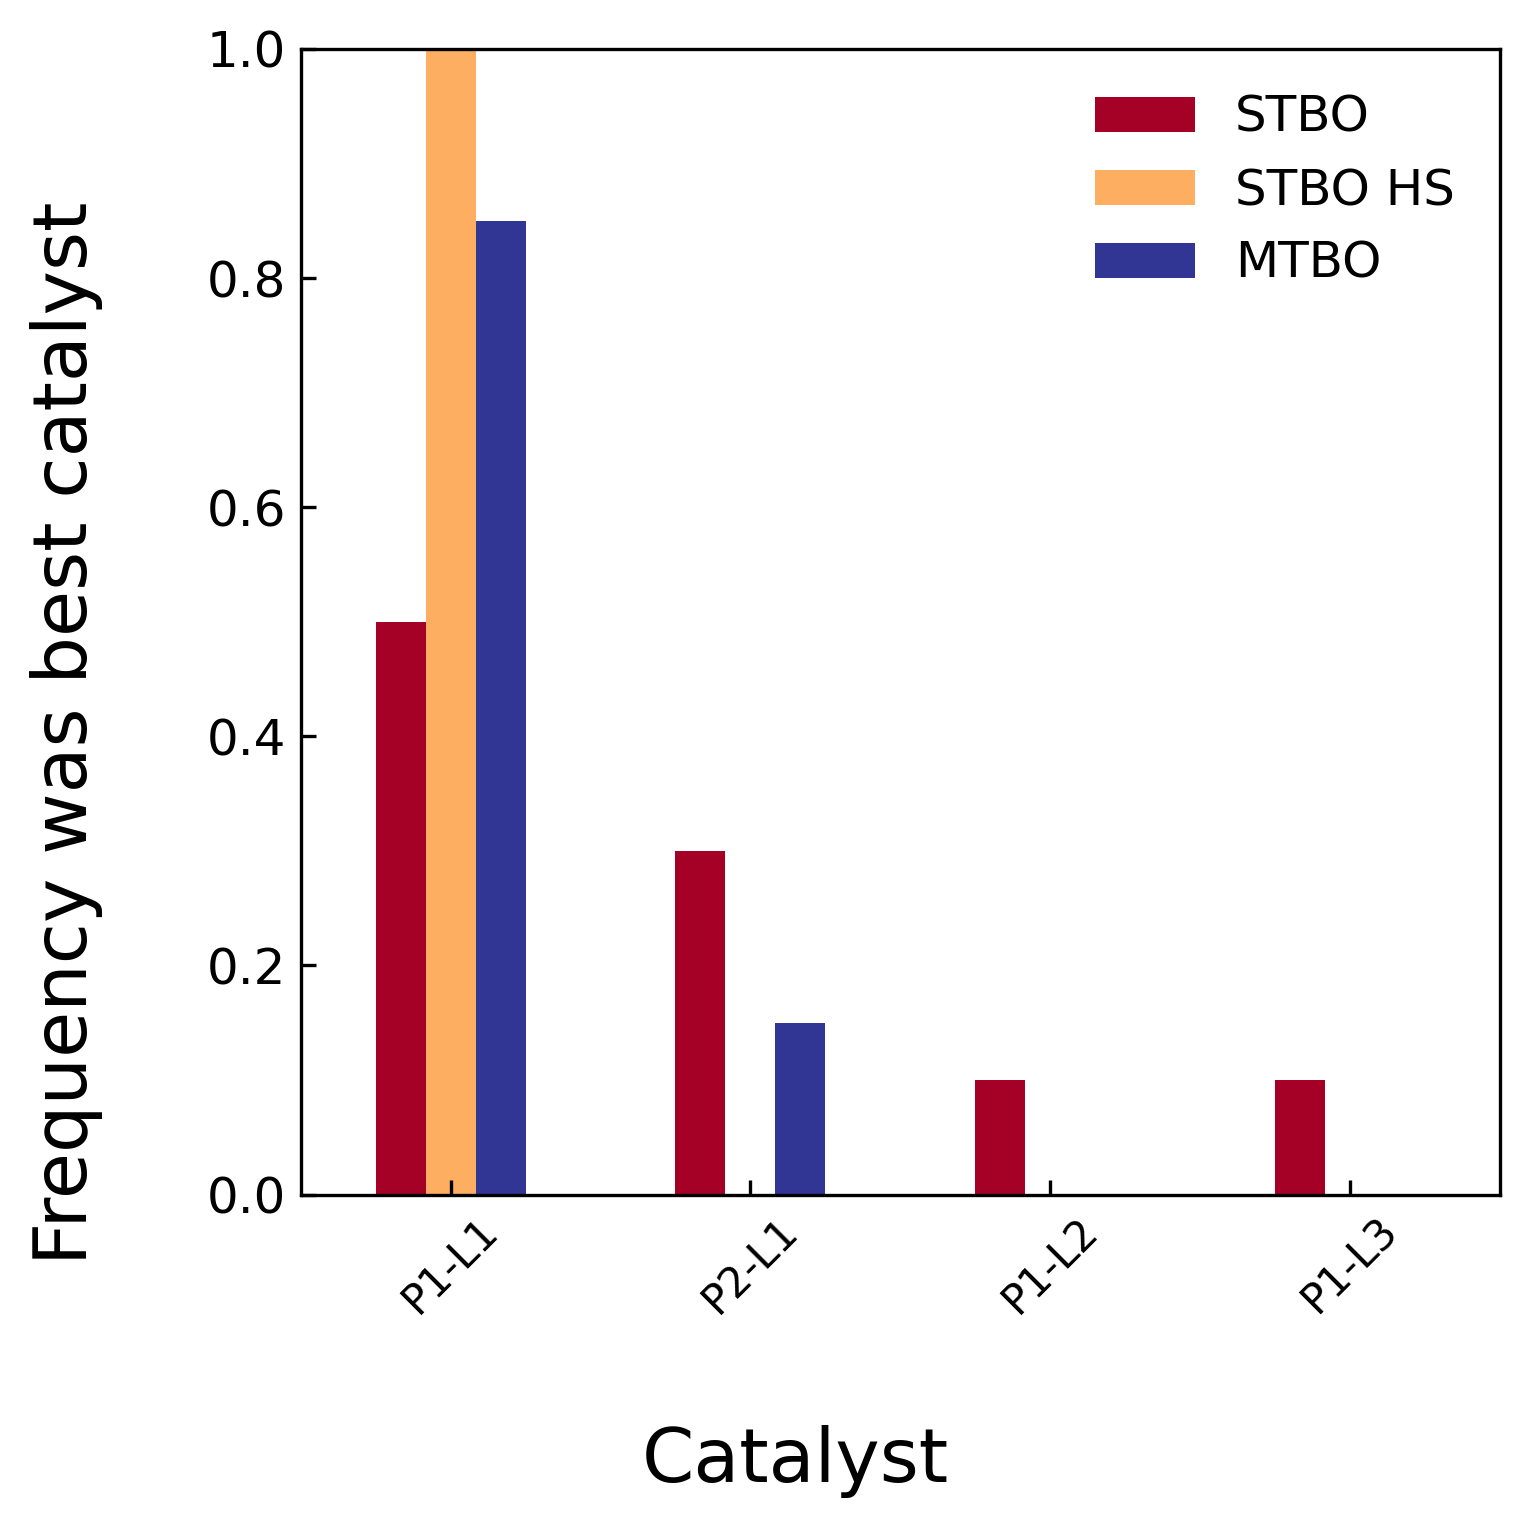
\includegraphics[width=0.8\linewidth]{gfx/Chapter03/baumgartner_suzuki_reizman_suzuki_all_cotraining_optimization_catalyst_best.png}
    \end{subfigure}
    \caption{ A comparison of the performance of single-task Bayesian Optimization (STBO), STBO head start (STBO HS), and multi-task Bayesian Optimization (MTBO) of Suzuki B1 and all of Suzuki R1-R4 as auxiliary tasks. (a)  The average best yield with a 95 \% confidence interval over 20 repeats is shown.  (b) Frequency of selection of each catalyst in Scheme 1 by STBO and MTBO.}
    \label{fig:baumgartner_suzuki_reizman_suzuki_all_cotraining_optimization}
\end{figure}

Here, STBO HS also performs well, suggesting that the optimal conditions from the auxiliary task are highly transferable to the new task. The success of STBO HS, however, shows that the similarity between tasks matters significantly for transfer learning. Therefore, in the next section, we explore benchmarks where we can finely tune the similarity between tasks to better understand what drives the success of MTBO.

These simulated case studies suggest that the use of MTBO is often beneficial, particularly when not mapping the predicted reactivity differences of the main and auxiliary substrates \textit{a priori}. Initial guesses (optimization starting points) are typically better than random initialization because of previous reaction information, and the rate of `best yield' improvement is also greater. In the best-case scenario, the reactivity of the new substrate is similar to those of previous datasets and results in a greater yield much faster than standard STBO. In the worst-case scenario, MTBO can fail with one noisy auxiliary case, but we found that using multiple auxiliary tasks helps to mitigate these issues.  With these findings, we were confident that MTBO would be effective in real-world case studies where we have experimental datasets from previous optimization campaigns. Further \textit{in silico} case studies for other reaction types, namely Buchwald-Hartwig cross couplings, were also conducted and showed similarly promising results; these studies can be found in the \ref{benchmarking_appendix}.

\subsection{Experimental Case Studies: C-H Activation}

The reaction class that we targeted for our experimental MTBO study was the palladium-catalyzed C-H activation reaction, reported by Hennessy and Buchwald, yielding pharmaceutically relevant oxindoles (\textbf{16}) from their corresponding chloroacetanilides (\textbf{15}), as shown in Figure \ref{fig:ch_activation}. Each case study is highlighted if it is forming a potential bioactive fragment or active pharmaceutical ingredient (API) intermediate. The rationale behind these studies is two-fold: firstly, these oxindoles are closely related to many known bioactive molecules and hence medicinal chemistry projects, and secondly, when considering optimal growth vectors for bioactive molecular fragments to grow into more potent drug candidates (such as in FBDD), the most beneficial transformations are often exploiting C--H bonds on the fragment to form new C--C bonds. Therefore, using MTBO, we aimed to rapidly optimize several transformations using different starting materials with unique functionalities to yield structurally diverse oxindole products by forming valuable sp\textsuperscript{2}-sp\textsuperscript{3} C--C bonds. Then, for future optimization campaigns requiring oxindole syntheses, this model can be employed to expediate reaction optimization and process development for new substrates.

\begin{figure}
    \centering
    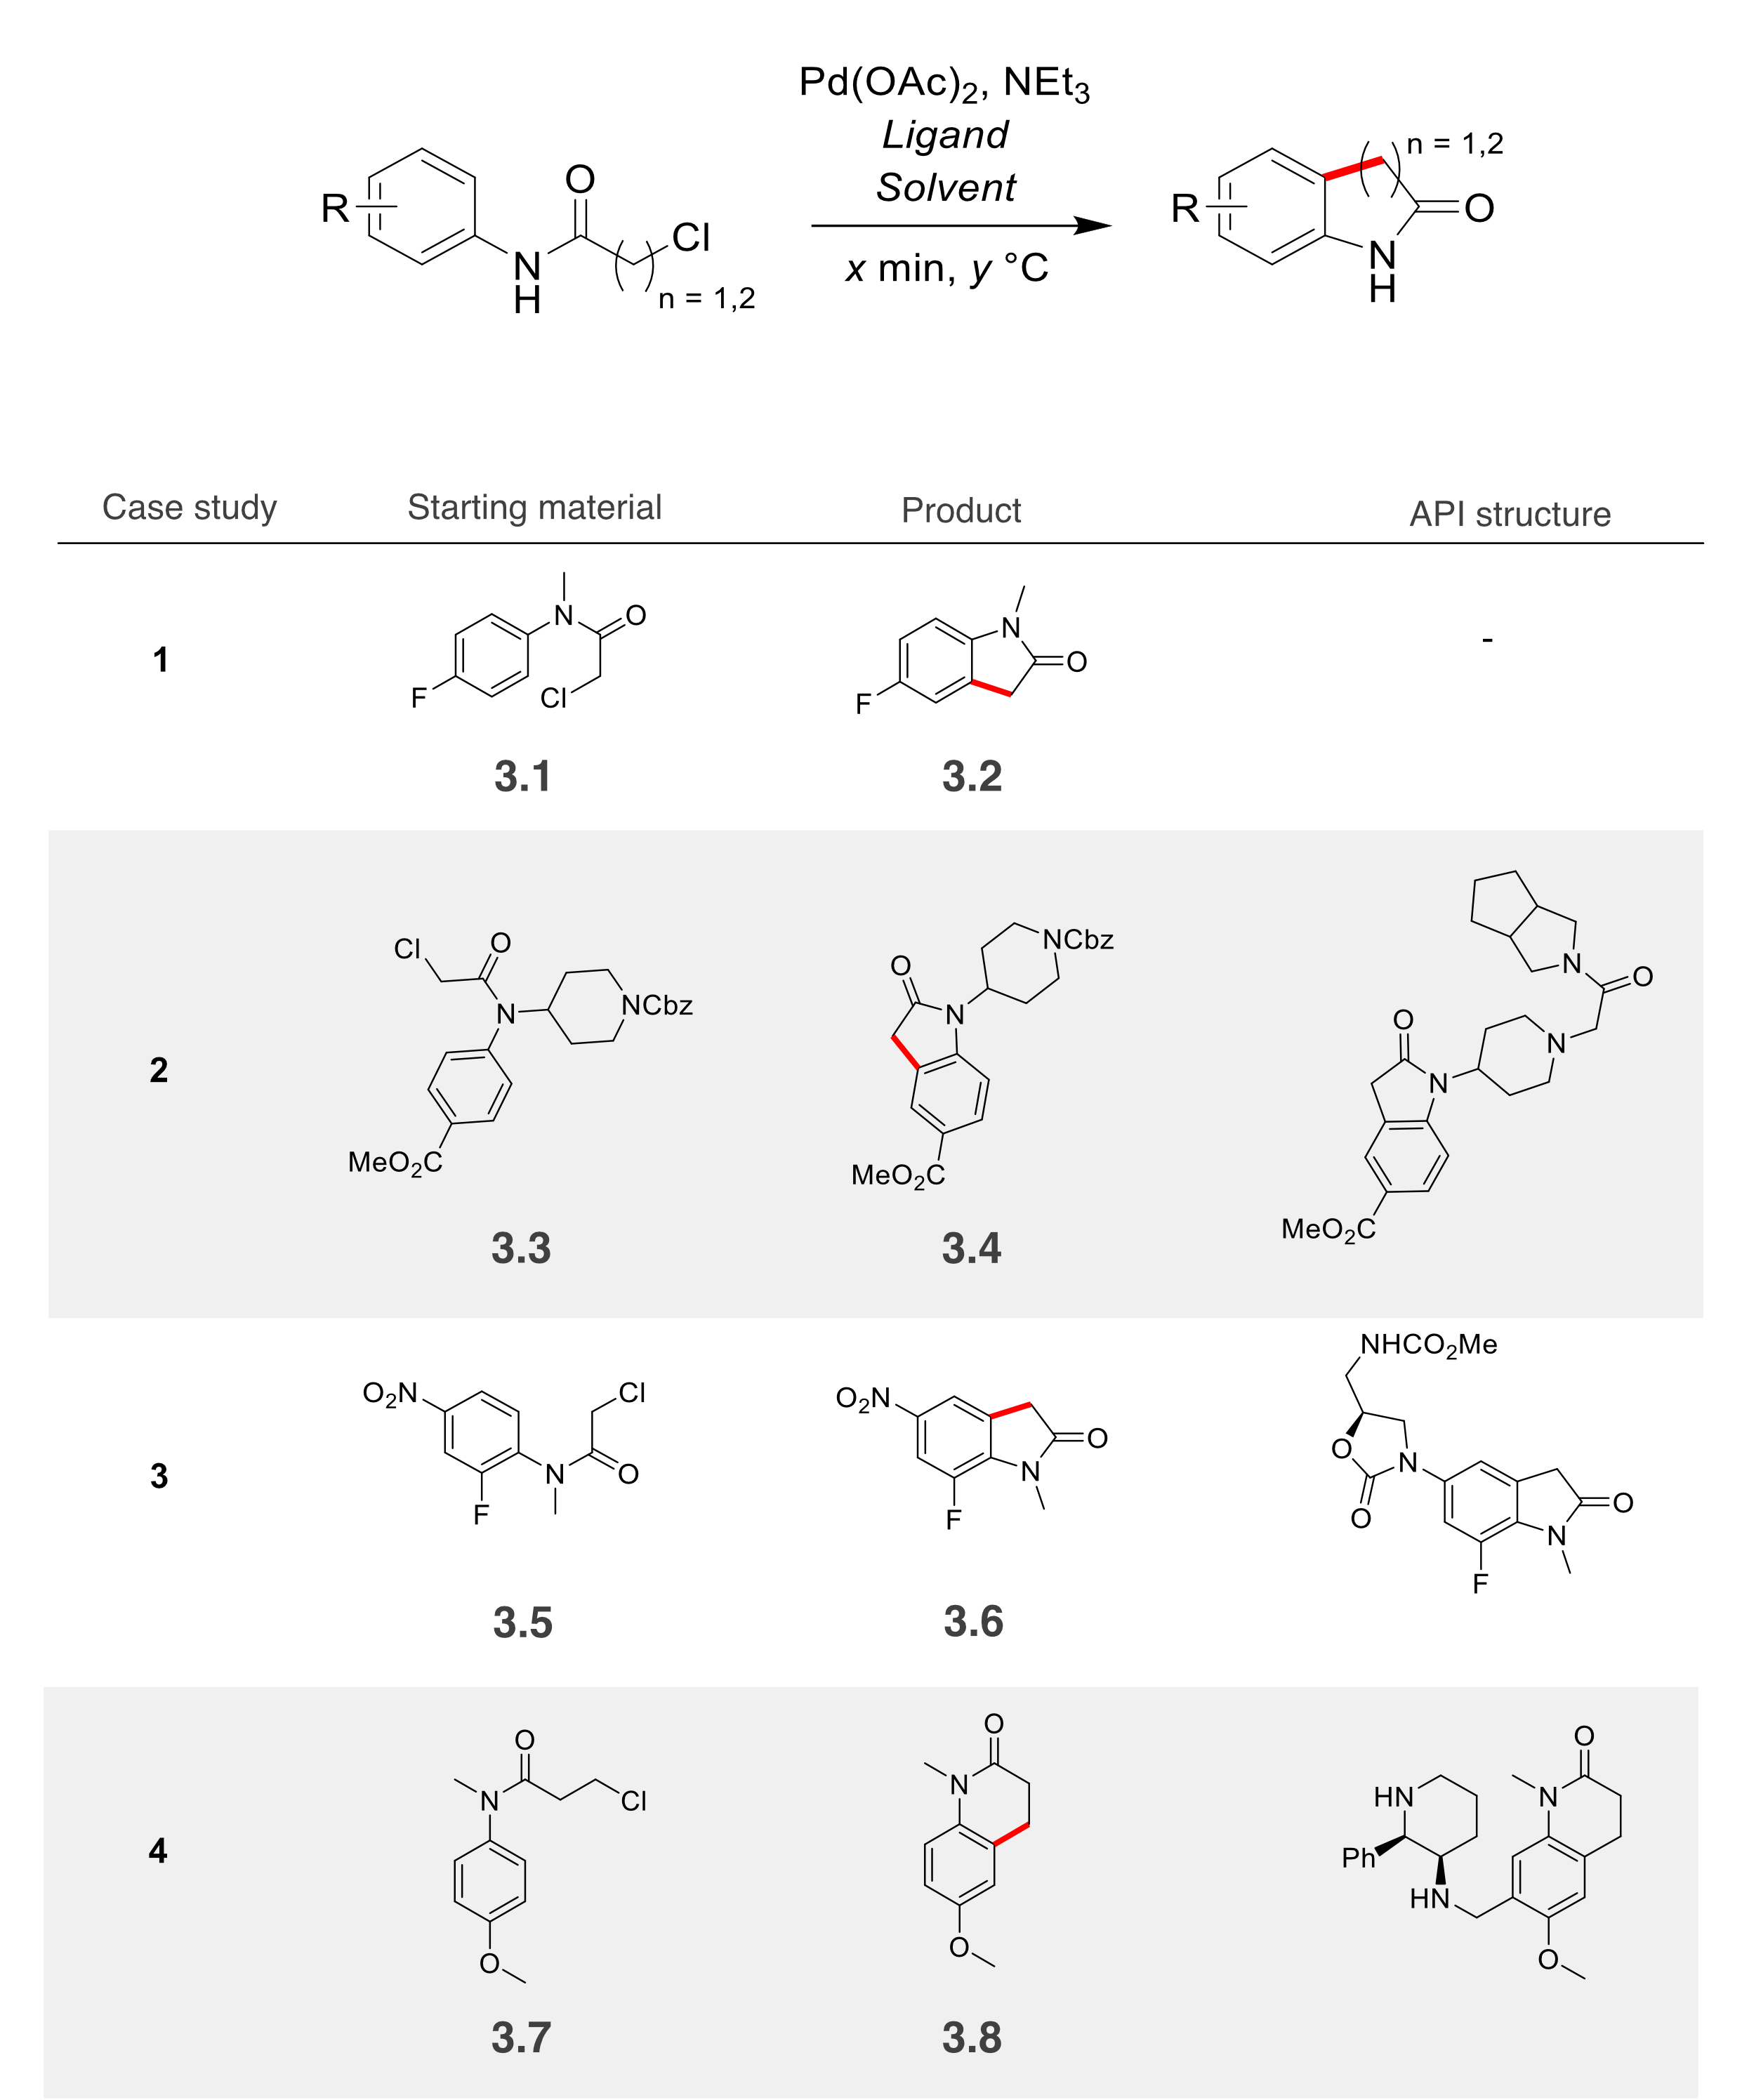
\includegraphics[width=\textwidth]{gfx/Chapter03/ch_activation_case_studies.png}
    \caption{ The reaction class of interest for the MTBO study, where the substituted chloroacetanilide, \textbf{15}, reacts to form the corresponding oxindole, \textbf{16}. Pd(OAc)\textsubscript{2} and NEt\textsubscript{3} remain constant in each experiment, but the ligand, solvent, catalyst concentration, residence time and reaction temperature are optimized for each case study. Each experimental case study explored in this work, including the starting material used, the product formed and the API structure that the product is linked to. These reactions, and references to their known API structure, are highlighted in Schemes 3 - 6}
    \label{fig:ch_activation}
\end{figure}

For all experimental work conducted during this study, a self-optimizing flow reactor platform was utilized with a control interface previously disclosed by our group. This platform employs an autonomous optimization workflow, where all experiments are conducted and analyzed without human intervention. All initial training experiments are planned using LHS, then the results from these automated experiments (the yield of the product) are exported using on-line HPLC sampling. This LHS step is only present when there is no previous experimental information for MTBO to learn from. Based on these reaction data, and any previously conducted auxiliary tasks, the MTBO algorithm then determines the most beneficial reaction conditions to execute in order to maximize product yield. The actual product yield obtained from this reaction is then communicated back to the algorithm, where the experimental feedback loop is closed, as the algorithm suggests conditions for the next optimization iteration (as shown in in Figure \ref{fig:self_opt_setup}). Furthermore, only minimal amounts of reaction material are consumed in each experiment by using reaction slugs; this is an important miniaturization consideration relevant to medicinal chemistry settings, but could potentially be miniaturized further. The minimum slug length is determined on the basis of dispersion in laminar flow such that sampling from a slug is consistent between slugs in repeated tests - the volume of the slugs used in these studies is 4 - 6 mL. This slug volume is determined by the Vapourtec Flow Commander software and varies depending on the necessary solvent dilution. The aim of this experimental methodology is to accelerate the optimization timeline by requiring fewer experiments and less reaction material consumption. More information on the reactor setup can be found in the Methods section.

\begin{figure}
    \centering
    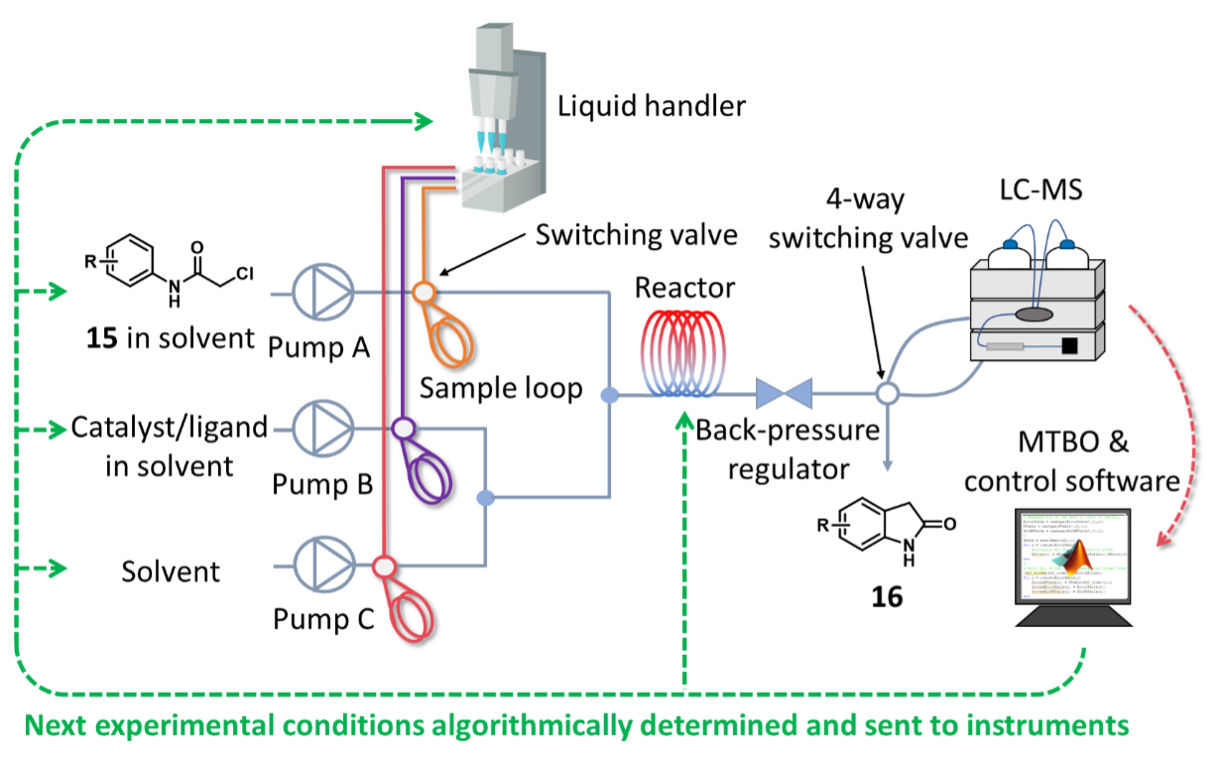
\includegraphics{gfx/Chapter03/self_optimization_setup.png}
    \caption{A schematic diagram of the experimental setup and protocol we used for the MTBO self-optimization studies.}
    \label{fig:self_opt_setup}
\end{figure}

For each case study, we optimized the continuous parameters: residence time (5 - 60 minutes), reaction temperature (50 - 150 °C) and catalyst concentration (1 - 10 mol\%), and the categorical parameters: solvent (toluene, DMA, acetonitrile, DMSO, NMP) and ligand (JohnPhos, SPhos, XPhos, DPEPhos), for the maximum product yield output. While it is possible to represent these categorical variables in numerous ways, the simplest representation (one-hot encoding) proved sufficient to learn from. The first case study, utilizes only single-task Bayesian optimization (STBO) as there is no previous data to leverage model understanding for MTBO. The starting material, \textbf{3.1}, reacts to form the molecular fragment (with potential growth vectors for further functionalization), \textbf{3.2}. The optimization was initialized using 16 training experiments before the algorithm began to suggest experimental conditions. We subsequently optimized case study two, three and four with the experimental data from the previous case studies as separate tasks.

For each of these consecutive C-H activation case studies, iteratively fewer experiments were (generally) necessary to achieve an optimal set of reaction conditions for the highest process yields - this is illustrated in Figure \ref{fig:optimization_curves}. This is because there was an increasing data-density that detailed optimal areas of parameter space for similar tasks (reactions of similar substrates), allowing for a progressively more efficient optimization workflow. In each case study, only minimal amounts (for our specific reaction system) of starting materials were consumed to find optimal reaction conditions, which is very important in early-stage medicinal chemistry development applications when preservation of precious starting materials and speed of optimization are paramount. For these C--H activation case studies, utilizing this workflow with MTBO to find optimal reaction conditions resulted in a material saving of 132 g (£25k) when compared with kinetic studies, and a material saving of 167 g (£32k) when compared with traditional DoE optimization studies (see ESI for details). These costly figures indicate why intermediate reaction optimization in medicinal chemistry applications are often difficult or infeasible to conduct, and why MTBO can serve as an enabling tool for these scenarios. Other common optimization strategies, such as traditional one-factor at a time (OFAT) approaches, may provide modest process improvements in these scenarios but have been shown repeatedly to underperform when compared with statistical-based techniques. This methodology has therefore proven to be effective in real-world pharmaceutical applications for material- and cost-efficiency, with the bonus of full automation that allows scientists to use their human resource to focus on other areas of chemical development. Although these experimental studies focused on C--C bond formation by targeting C--H activation, these techniques can be utilized for other transformations to ultimately accelerate optimization.

\begin{figure}
    \centering
    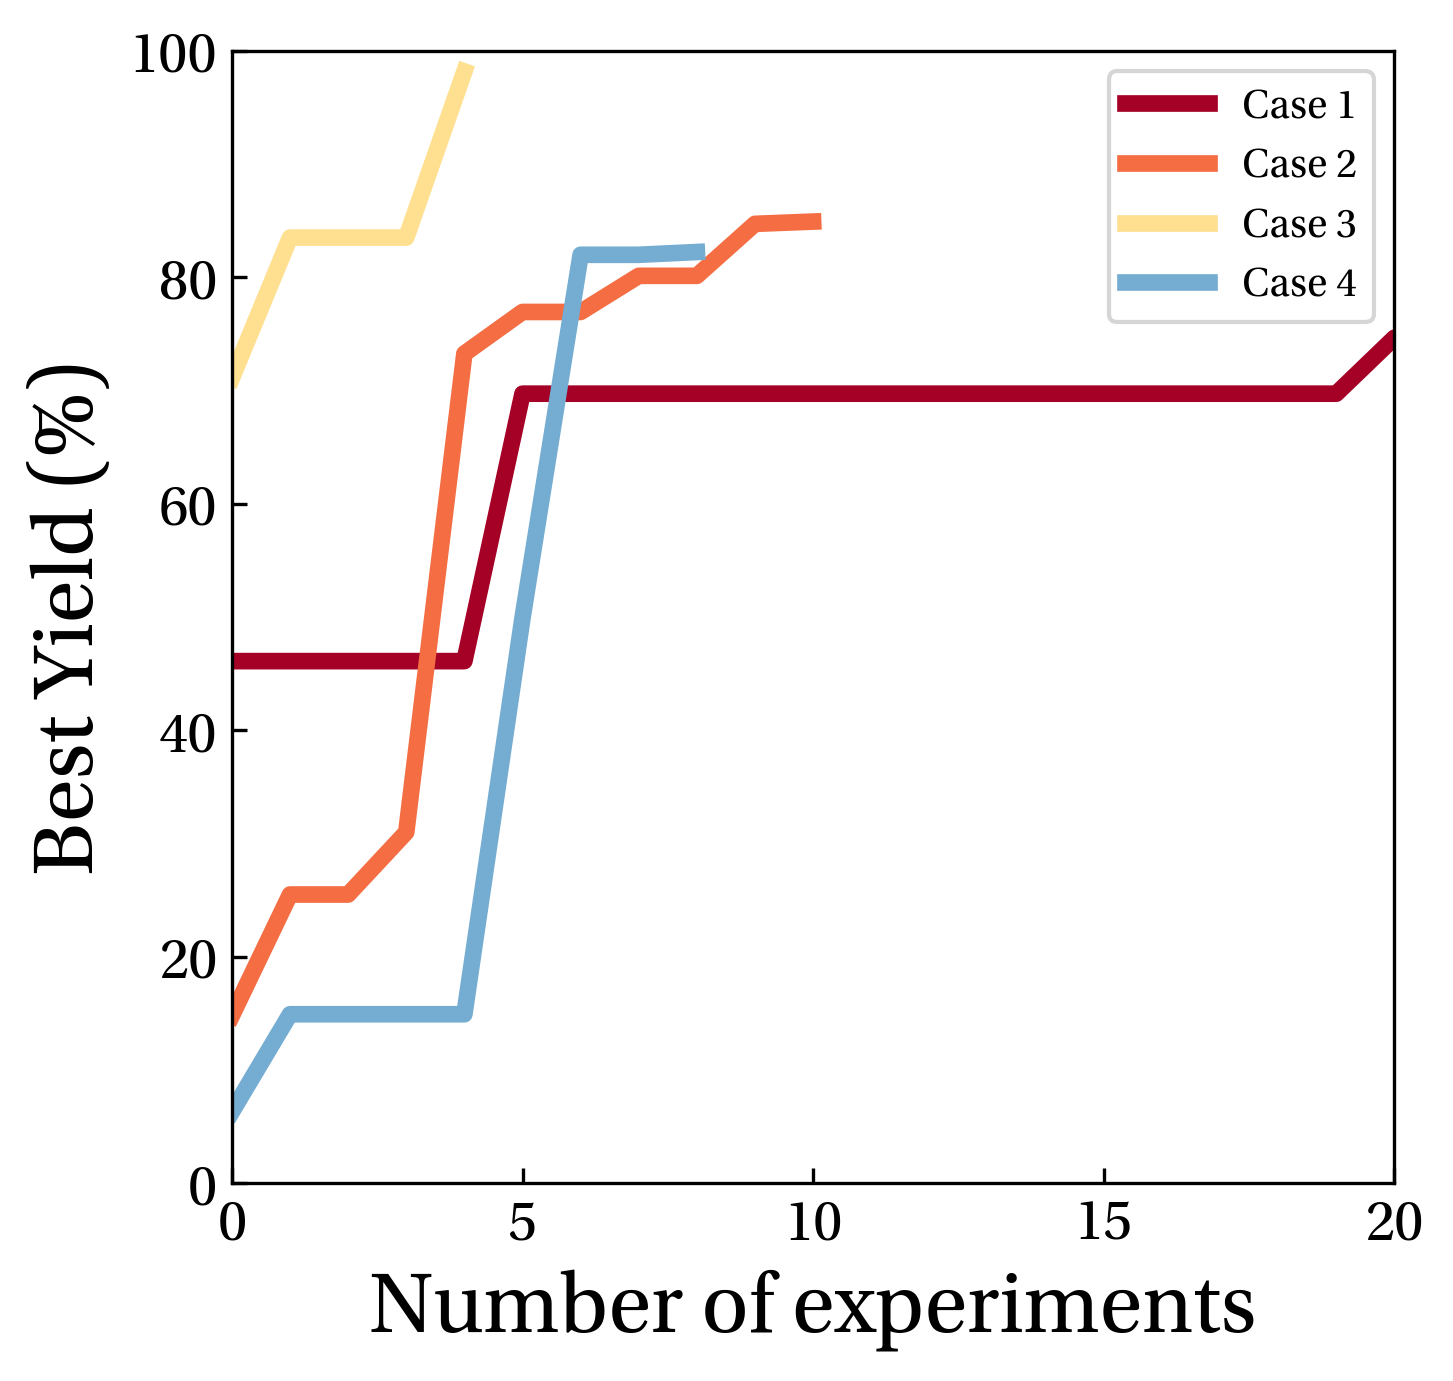
\includegraphics[width=\textwidth]{gfx/Chapter03/ch_activation_optimization_curves.png}
    \caption{A plot of best yield of the products in each case study against the optimization experimental number in each campaign.}
    \label{fig:optimization_curves}
\end{figure}


\section{Conclusions}

The studies performed in this work, both \textit{in silico} and in real-world chemical applications, represent the first use of datasets from similar reactions to expediate current optimization campaigns with multi-task Bayesian optimization. This methodology drastically shortens optimization timelines for pharmaceutically relevant transformations, whereas other traditional process optimization techniques (i.e. design of experiments, kinetics studies) would require a significantly higher investment in starting materials, time and cost. This would likely make their optimization infeasible in medicinal chemistry workflows and early-stage process development, unless using intuition-based optimization techniques (such as OFAT) that are unlikely to obtain optimal results. By introducing more miniaturization technology, including smaller reactors/slugs and plate-based screening, there is the added opportunity to reduce material consumption even further using these automated platforms.

With the increasing density of chemical reaction data, both in the literature and in private data storage, there is a wealth of information that can be leveraged for building task-specific models to further increase the efficiency of future reaction optimizations. When using these multi-task learning approaches, it is possible to generate sets of models for specific reaction classes (e.g. Buchwald-Hartwig, Suzuki etc.) and subsets of those models (electron-rich, sterically hindered etc.) to rapidly optimize any transformation likely to be encountered. This is a particularly powerful technique in cases where starting materials are sparse and the reaction is poorly understood, yet suitable quantities of product is required for further molecular design, functionalization and biological testing. Similarly, this importance is echoed in early process development when scale-up of a novel synthetic intermediate is required from the milligram scale to multi-gram or kilogram scale. The primary challenge when using multi-task Bayesian optimization is its tendency to bias towards the best conditions found in a single auxiliary task, as shown in our \textit{in silico} studies. However, our results demonstrate that additional useful auxiliary tasks can reduce the impact of a noisy, low-yielding auxiliary task. Future work could use a more exploratory acquisition function in combination with the multi-task model to strike the right balance between biasing towards the auxiliary task data and exploring untested conditions.

The multi-task Bayesian optimization algorithm used in this study is open-source and is released as a package within the Summit framework previously reported by our group. This step towards utilizing machine learning and previous reaction data for future optimization campaigns will ultimately result in faster and more efficient optimizations, thereby serving as a broadly applicable enabling tool with relevance to medicinal chemistry and FBDD settings, where industry-standard process optimization techniques are impractical or even impossible to implement.

\section{Methods}


\subsection{Multitask Bayesian Optimization}

Bayesian optimization (BO) is detailed in Chapter \ref{ch:summit}. Multi-task BO (MTBO) replaces the GP in Bayesian optimization with a multi-task GP. I use the intrinsic model of coregionalization originally proposed by Bonilla et al.,\cite{Bonilla2007} which defines a multi-task kernel $k^{ICM}_{\theta}$ as the Kronecker product of standard GP kernel (the Matérn kernel in our case) and a task kernel $k^t_{\theta}$:
\begin{equation}
    k^{ICM}_{\theta}(x,x') = k^t_{\theta} \otimes  k_{\theta}(x,x')
\end{equation}
The task kernel $k^t_{\theta}$ is a $T \times T$ matrix of trainable parameters where $T$ is the number of tasks. These parameters represent the inter-task correlation.

\subsection{Benchmarks}
% Prior to real experimentation, we wanted to understand the performance of MTBO in simulated studies. We examined two literature reports that contain experimental results from Suzuki-Miyaura coupling reactions,\cite{Baumgartner2018, Reizman2016b} and one report with results from a Buchwald-Hartwig cross-coupling[51] (demonstrated in the Supporting Information), building a predictive model for the reaction yield to behave as the ground-truth for simulated optimization studies. Buchwald-Hartwig and Suzuki-Miyaura couplings are ubiquitous in the pharmaceutical and fine chemicals industries as they allow rapid construction of aromatic scaffolds through reactions with few impurities.[52] We therefore chose these reaction classes because of their high value and applicability to real-world scenarios. More details on benchmark training can be found in the Appendix.

We used literature data to benchmark our strategies \textit{in silico}. The challenge is that chemical data is often recorded in unstructured text documents such as journal publications and patents. While there are some conventions, each author is free to express the details of a chemical reaction as they wish. Such unstructured information is not amenable to most machine learning algorithms. Therefore, we designed a custom data extraction workflow that we think is a model for how to apply transfer learning in chemistry.

As shown in Figure \ref{fig:ord_pipeline}, our workflow that converts unstructured data into benchmarks that can be used for comparing various strategies.  We leveraged the Open Reaction Database (ORD) format as a common representation of reactions \cite{Kearnes2021}. We wrote converters from spreadsheet formats to ORD. Once the data was transformed into ORD, the data was loaded into local storage on disk. Subsequently, the featurization step turned the ORD schema into a set of features that can be used for training a benchmark or a GP for Bayesian Optimization.  We used one-hot encodings to represent the categorical variables. 

\begin{figure}[t]
    \centering
    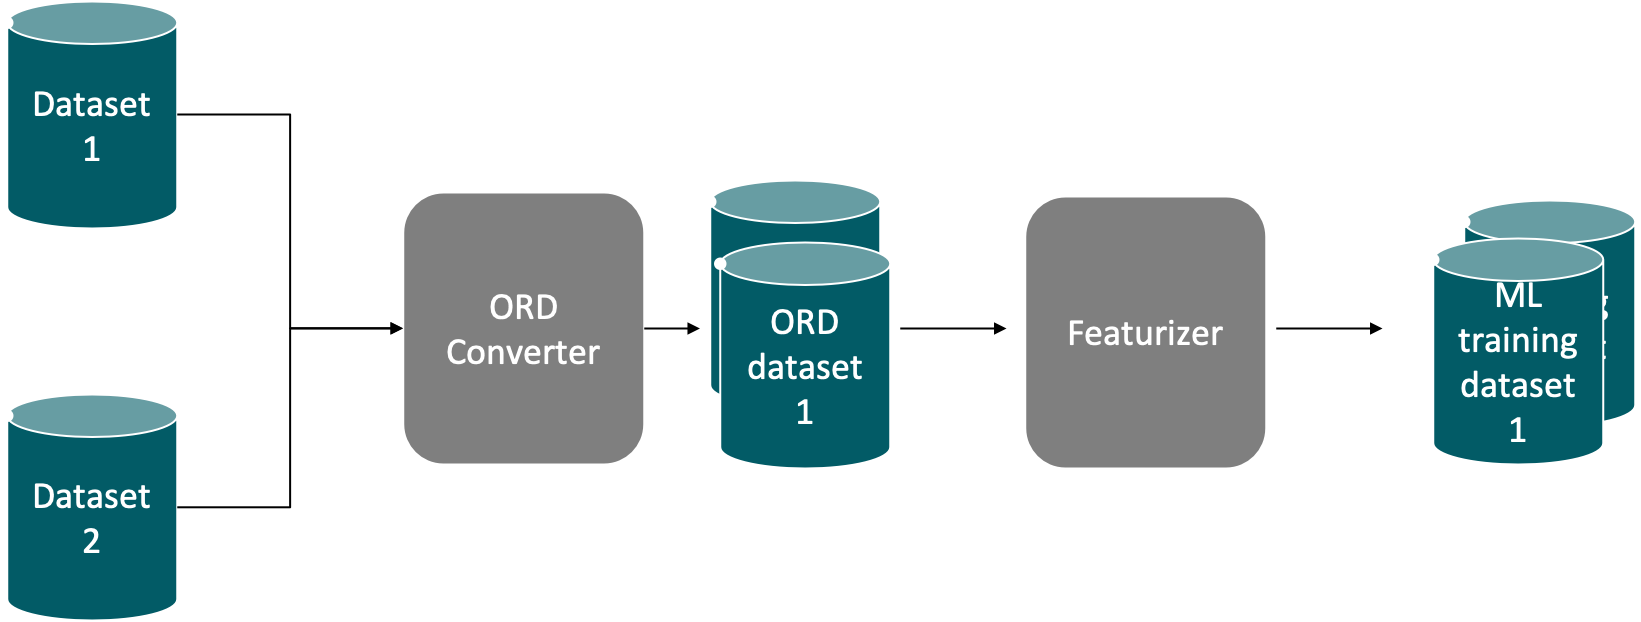
\includegraphics[width=\textwidth]{gfx/Chapter03/etl_pipeline.png}
    \caption{Diagram of a pipeline for turning raw data from the literature into a standard intermediate schema, which can be used to generate features for downstream machine learning tasks.}
    \label{fig:ord_pipeline}
\end{figure}

We examined two literature reports that contain experimental results from Suzuki-Miyaura coupling reactions \cite{Baumgartner2018, Reizman2016b} ,and one report with results from a Buchwald-Hartwig cross-coupling \cite{Baumgartner2019}, building a predictive model for the reaction yield to behave as the ground-truth for simulated optimization studies. Buchwald-Hartwig and Suzuki-Miyaura couplings are ubiquitous in the pharmaceutical and fine chemicals industries as they allow rapid construction of aromatic scaffolds through reactions with few impurities \cite{Brown2016}. We therefore chose these reaction classes because of their high value and applicability to real-world scenarios. The specific reactions used are detailed in Figures \ref{fig:benchmarks_cn} and \ref{fig:benchmarks_suzuki}.


\begin{figure}
    \centering
    
\includegraphics[width=0.9\textwidth]{gfx/Chapter03/c_n_benchmarks_thesis.png}
    \caption{Benchmark examples of C-N cross coupling (C-N B1-B4) of nitrogen functionalized aromatics (1, 4, 6, 8) with p-tolyl triflate. Data is based on experiments by Baumgartner et al. 
 \cite{Baumgartner2019}. The base equivalents, temperature and reaction time, base and catalyst are varied to maximize yield.}
    \label{fig:benchmarks_cn}
\end{figure}



We leveraged Summit to build the predictive models from the literature reports. We utilized the ExperimentalEmulator feature in Summit, which creates a benchmark based on experimental data. The regressor used was a neural network with one hidden layer of 512 units with a ReLu activation function. A one-hot encoding was used for the pre-catalyst and ligand combinations. The neural networks were trained by five-fold cross validation over 1000 epochs using stochastic gradient descent. See Appendix 1 for the parity plots for the benchmarks. 

\subsection{Flow Reactor Platform}

The reactor platform consists of two Vapourtec R2 modules for controlling flow rates, a Vapourtec R4 reactor module for controlling reactor temperature, a Gilson GX-271 liquid handler for dispensing and collecting reaction material and LC-MS analytical equipment (Shimadzu/Waters) for reaction outcome determination. The Vapourtec R2 modules are connected using 30 cm sections of 1 mm ID stainless steel tubing and T-pieces, entering a Vapourtec stainless steel reactor (10 mL volume) and exiting via a 50-bar back pressure regulator and a 80 cm section of 1 mm ID stainless steel tubing to a switching valve. For each reaction, with the experimental conditions determined through LHS or algorithmically, the liquid handler dispenses 2 mL slugs of the starting material (in this case, the chloroacetanilide) pre-dissolved in the selected solvent into the sample loop for pump A - this solution also contains biphenyl as an internal standard. The selected catalyst/ligand combination in the same solvent is then loaded into the sample loop for pump B, and the solvent of interest is loaded into pump C for dilution. The reaction is conducted with a constant 0.09 M reactor concentration, yielding the corresponding product (in this case, the oxindole), which is thereby analyzed utilizing a 4-way switching valve for on-line LC-MS. Using this methodology, experiments can be run using only minimal amounts of reaction material for each experiment as we are utilizing reaction slugs. This experimental workflow is illustrated in Figure \ref{fig:self_opt_setup}.

%*****************************************
%*****************************************
%*****************************************
%*****************************************
%*****************************************
